\documentclass[journal=esthag,manuscript=article]{achemso}
%%%%%%%%%%%%%%%%%%%%%%%%%%%%%%%%%%%%%%%%%%%%%%%%%%%%%%%%%%%%%%%%%%%%%
%% Place any additional packages needed here.  Only include packages
%% which are essential, to avoid problems later. Do NOT use any
%% packages which require e-TeX (for example etoolbox): the e-TeX
%% extensions are not currently available on the ACS conversion
%% servers.
%%%%%%%%%%%%%%%%%%%%%%%%%%%%%%%%%%%%%%%%%%%%%%%%%%%%%%%%%%%%%%%%%%%%%
\usepackage[T1]{fontenc}       % Use modern font encodings
\usepackage[utf8]{inputenc}
\usepackage{todonotes}
\usepackage{amsmath}

%%%%%%%%%%%%%%%%%%%%%%%%%%%%%%%%%%%%%%%%%%%%%%%%%%%%%%%%%%%%%%%%%%%%%
%% If issues arise when submitting your manuscript, you may want to
%% un-comment the next line.  This provides information on the
%% version of every file you have used.
%%%%%%%%%%%%%%%%%%%%%%%%%%%%%%%%%%%%%%%%%%%%%%%%%%%%%%%%%%%%%%%%%%%%%
%%\listfiles

%%%%%%%%%%%%%%%%%%%%%%%%%%%%%%%%%%%%%%%%%%%%%%%%%%%%%%%%%%%%%%%%%%%%%
%% Place any additional macros here.  Please use \newcommand* where
%% possible, and avoid layout-changing macros (which are not used
%% when typesetting).
%%%%%%%%%%%%%%%%%%%%%%%%%%%%%%%%%%%%%%%%%%%%%%%%%%%%%%%%%%%%%%%%%%%%%
%% \newcommand*\mycommand[1]{\texttt{\emph{#1}}}


%%%%%%%%%%%%%%%%%%%%%%%%%%%%%%%%%%%%%%%%%%%%%%%%%%%%%%%%%%%%%%%%%%%%%
\author{Eduard Szöcs}
\affiliation[Institute for Environmental Sciences]{Institute for Environmental Sciences, University of Koblenz-Landau, Germany}
\email{szoecs@uni-landau.de}
\phone{+49 (0)6341 280 31552}

\author{Marvin Brinke}
\affiliation[German Federal Institute of Hydrology]{German Federal Institute of Hydrology (BfG), Koblenz, Germany}

\author{Bilgin Karaoglan}
\affiliation[German Federal Environmental Agency]{Federal Environmental Agency (UBA), Dessau-Roßlau, Germany}

\author{Ralf B. Schäfer}
\affiliation[University Koblenz-Landau]{Institute for Environmental Sciences, University of Koblenz-Landau, Germany}


%%%%%%%%%%%%%%%%%%%%%%%%%%%%%%%%%%%%%%%%%%%%%%%%%%%%%%%%%%%%%%%%%%%%%
\title[Pesticides small streams]{Pesticides in small agricultural streams in Germany}
% \abbreviations{mo, neon, ra, tu, fw}
\keywords{Monitoring, Neonicotinoid, Risk Assessment Toxic Units, Freshwater}
% RAC, 

%%%%%%%%%%%%%%%%%%%%%%%%%%%%%%%%%%%%%%%%%%%%%%%%%%%%%%%%%%%%%%%%%%%%%
\begin{document}
%%%%%%%%%%%%%%%%%%%%%%%%%%%%%%%%%%%%%%%%%%%%%%%%%%%%%%%%%%%%%%%%%%%%%
%% The "tocentry" environment can be used to create an entry for the
%% graphical table of contents. It is given here as some journals
%% require that it is printed as part of the abstract page. It will
%% be automatically moved as appropriate.
%%%%%%%%%%%%%%%%%%%%%%%%%%%%%%%%%%%%%%%%%%%%%%%%%%%%%%%%%%%%%%%%%%%%%
\begin{tocentry}

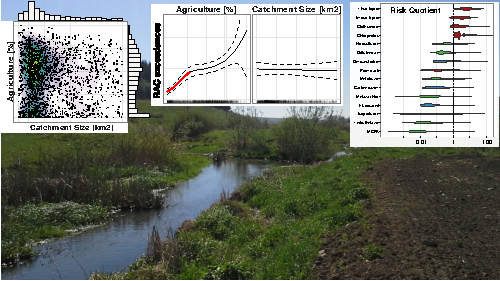
\includegraphics[width=0.7\textwidth]{abstract.pdf}

\end{tocentry}



%%%%%%%%%%%%%%%%%%%%%%%%%%%%%%%%%%%%%%%%%%%%%%%%%%%%%%%%%%%%%%%%%%%%%
\begin{abstract}
% 150-200 words
Small streams are important refugia for biodiversity.
In agricultural areas, they may be at high risk of pesticide pollution. However, most related studies have been limited to a few streams on the regional level, hampering extrapolation to larger scales.
In Germany, pesticide monitoring is performed by the federal states as part of water quality surveillance. The related data also cover small streams and may contribute to national-scale risk assessment.
% * <ralf.schaefer@aggiemail.usu.edu> 2016-08-26T13:30:31.255Z:
%
% Chemical status is misleading because pesticides are largely riverbasin specific pollutants and therefore are dealt with as complementary parameter for the ecological status
%
% ^.

We compiled monitoring data focusing on small streams, resulting in a data set of 2,918,604 measurements from 42,236 samples in 3,049 sampling sites covering the years 2005-2014.
A total of 484 different compounds that can be classified as pesticides were measured.
Especially neonicotinoid insecticides and Chlorpyrifos showed exceedances of regulatory acceptable concentrations (RACs). We found a lack of data for small streams \textless 10 km\textsuperscript{2} catchment size. This, and the heterogeneity between the federal state monitoring programs, hampered a nation-scale assessment.
% * <ralf.schaefer@aggiemail.usu.edu> 2016-08-26T13:35:37.869Z:
%
% Mehr inhaltliche ERgebnisse wären gut
%
% ^ <ralf.schaefer@aggiemail.usu.edu> 2016-08-26T15:17:05.687Z:
%
% Hm - widerspricht sich auch mit dem Scope oben/storyline... Würde ich positiver formulieren, Despite heterogeneity etc. the data show that...
%
% ^.
Our result suggest that pesticides originating from agricultural land use might be a major threat for aquatic ecosystems.
% * <ralf.schaefer@aggiemail.usu.edu> 2016-08-26T15:17:24.497Z:
%
% paar mehr details wären gut hier, fällt etwas vom himmel die schlussfolgerung
%
% ^.
The exceedances of RACs indicate risks originating from few compounds.
However, future monitoring programs need to be unified between states to provide more reliable assessments. \todo{Letzter Absatz gefällt mir nicht...}
% * <ralf.schaefer@aggiemail.usu.edu> 2016-08-26T15:18:34.357Z:
%
% letzer absatz sehr wirr. Schlage folgende Struktur vor: 3-4 SÄtze zu Ergebnissen, ohne Interpretation und dann einen Satz Schlussfolgerung
%
% ^.

%182 words
\end{abstract}


%%%%%%%%%%%%%%%%%%%%%%%%%%%%%%%%%%%%%%%%%%%%%%%%%%%%%%%%%%%%%%%%%%%%%
\section{Introduction}

More than 50\% of the total land area in Germany are used by agriculture \citep{statistisches_bundesamt_bodenflache_2014}.
In the year 2014 more than 45,000 tonnes of 766 authorized pesticides were sold for application on this area \citep{bundesamt_fur_verbraucherschutz_und_lebensmittelsicherheit_absatz_2015}.
The applied pesticides may enter surface waters via spray-drift, edge-off-field run-off or drainage, with run-off being one of the major input routes \citep{schulz_comparison_2001,liess_determination_1999}.
% * <ralf.schaefer@aggiemail.usu.edu> 2016-08-27T11:54:54.730Z:
%
% da unten regenanalysen kommen, sollte hier noch was zu precipitation hinzugefügt werden
%
% ^.
Once entered the surface waters pesticides are frequently detected in environmental monitoring \citep{malaj_organic_2014} and may have adverse effects on biota and ecosystem functioning \citep{schulz_field_2004, schafer_effects_2007}.
% * <ralf.schaefer@aggiemail.usu.edu> 2016-08-27T10:58:27.621Z:
%
% besser zitieren: schäfer et al. 2012 thresholds ES&T - ist stärker, da mehr studien drin
%
% ^.
% * <ralf.schaefer@aggiemail.usu.edu> 2016-08-27T10:39:38.645Z:
%
% Der Einschub "frequently detected in .. monitoring" passt hier nicht so richtig hin
%
% ^.

\citet{malaj_organic_2014} analyzed data supplied to the European Union (EU) in the context of the Water Framework Directive (WFD) and showed that almost half of European water bodies are at risk from organic toxicants, with pesticides playing a major role.
However, this study reflected only a small part of data that is available in national monitoring programs.
These programs are setup to determine the pesticide pollution of surface, ground and drinking water.
% * <ralf.schaefer@aggiemail.usu.edu> 2016-08-26T15:24:18.962Z:
%
% hier schon spezifischer werden: Nur auf Pestizide beziehen
%
% ^.
Large amounts of data are generated, which possibly can also be used to answer other questions.
In Germany monitoring programs are setup independently by the federal states in compliance with the WFD \citep{quevauviller_water_2008} and additional state specific needs.
However, currently there is no curated national-wide compilation of this data available.
% * <ralf.schaefer@aggiemail.usu.edu> 2016-08-27T10:44:09.240Z:
%
% Letzter Abschnitt etwas schwach. Es wäre besser einer Struktur zu folgen: Malaj - Pestizide in EU. Nicht gesamte Daten. Situation Deutschland sollte noch enger verknüpft werden, warum SPrung  zu Deutschland. Eine mögliche Storyline wäre:  Malaj und Stehle & Schulz zeigen, dass vermutlich Belastung vorhanden. EU fordert keine einbussen an biodiversität (sustainable use directive). Unklar, wie repräsentativ bisherige Studien sind. Weitere Daten sind verfügbar. IN Bezug auf Biodiv spielen vor allem Kleingewässer eine Rolle usw.
%
% ^.

\citet{stehle_pesticide_2015} compiled 1566 measured concentrations of 23 insecticides in the EU from scientific publications. 
They found that many of these measurements exceed regulatory acceptable concentrations (RAC), especially in very small catchments \textless $1~km^2$.
Small water bodies are important refuges of biodiversity \citep{davies_comparison_2008} and enable downstream colonization of polluted streams \citep{liess_analyzing_2005}.
% * <ralf.schaefer@aggiemail.usu.edu> 2016-08-27T10:59:21.077Z:
%
% besser orlinskyi 2015 STOTEN, das bezieht sich direkt auf wiederbesiedelung
%
% ^.
At the same time they are at high risk of pesticide contamination from adjacent agricultural areas and low dilution effects \citep{liess_determination_1999}.
% * <ralf.schaefer@aggiemail.usu.edu> 2016-08-27T11:01:01.458Z:
%
% schulz 2004 beinhaltet auch direkt das verhältnis von größe und exposition
%
% ^.
% * <ralf.schaefer@aggiemail.usu.edu> 2016-08-27T11:00:32.608Z:
%
% sind ja keine 2 unterschiedlichen punkte - besser präzisieren
%
% ^.
Although small streams comprise a major fraction of streams \citep{nadeau_hydrological_2007}, relatively little is know about their chemical and ecological status.
% * <ralf.schaefer@aggiemail.usu.edu> 2016-08-27T11:01:43.074Z:
%
% ich würde diese WFD Begriffe vermeiden - chemical status im WFD Kontext beinhaltet gerade nicht die meisten Pestizide
%
% ^.

We compiled a large data set with chemical monitoring data for Germany and aimed to answer the following research questions: \\
(i) Can the currently available monitoring data be used for a representative description of the pollution situation? \\
(ii) Are small agricultural waters more polluted compared to bigger streams? Are there thresholds in these relationships? \\
% * <ralf.schaefer@aggiemail.usu.edu> 2016-08-27T11:05:01.605Z:
%
% welche relationships? Wird hier nicht klar
%
% ^.
% * <ralf.schaefer@aggiemail.usu.edu> 2016-08-27T11:04:12.011Z:
%
% wir haben ja gerade für große gewässer gar nicht alle daten gesammelt und können dsa doch gar nicht direkt beantworten
%
% ^.
(iii) How polluted are small streams and which pesticides are most important? Is the current approval process protective for these streams?  
% * <ralf.schaefer@aggiemail.usu.edu> 2016-08-27T11:29:55.457Z:
%
% Ich muss mal weiter lesen, aber einige der Fragen scheinen mir nicht beantwortet werden zu können. Z.b. Approval process - da wäre ja die Frage, ob die RACs ökologisch protektiv sind, dazu können wir nichts sagen... Du meinst wahrscheinlich was anderes
%
% ^.


\section{Methods}
\subsection{Data compilation}

We queried pesticide monitoring data from sampling sites with catchment sizes $\mathrm{< 100km^2}$ for the years 2005 to 2015 from all 13 non-city federal states of Germany. We will refer to the states using the ISO 3166-2:DE standard abbreviations.
Additionally, we compiled data available from previous studies and searched online databases.
% * <ralf.schaefer@aggiemail.usu.edu> 2016-08-27T11:34:07.673Z:
%
% zu unpräzise - mittlerweile muss man schon fast die genauen search terms angeben und bleibt auch unklar, was für zusätzliche Datensätze gesucht wurden. Tauchen die überhaupt auf? Wenn es nur Monitoringdaten sind, ist das eigentlich nicht wichtig
%
% ^.
This yielded to a total of more then 30 datasets of different formats.
% * <ralf.schaefer@aggiemail.usu.edu> 2016-08-27T11:36:48.417Z:
%
% entweder übersicht erstellen oder weglassen
%
% ^.

We homogenized and unified these datasets into a common database.
We implemented a robust and reproducible data cleaning work flow (Supplement, Figure S1) \citep{poisot_best_2015}, though parts of the dataset are proprietary.
% * <ralf.schaefer@aggiemail.usu.edu> 2016-08-27T11:37:21.589Z:
%
% was hat das cleaning mit dem proprietary zu tun?! Das soll eher sagen, dass man die daten nicht rausgeben kann und nicht für alle reproducible ist?
%
% ^.
An overview of the data cleaning process is provided in the supplemental materials.  
% * <ralf.schaefer@aggiemail.usu.edu> 2016-08-27T11:38:14.386Z:
%
% spezfischere angabe notwendig - kann aber eh in vorherigen Satz (for details see ...)
%
% ^.
To assess whether samples were taken during potential rainfall events we performed spatio-temporal intersection of sampling events with daily precipitation data from the sampling date and the day before. \citep{rauthe_central_2013}.
% * <ralf.schaefer@aggiemail.usu.edu> 2016-08-27T11:52:22.627Z:
%
% Das müsste ausführlicher beschrieben werden. Zunächst vielleicht mal 2 Sätze wie All sites  were georeferenced and transformed to the same CRS . Subsequently, each site was assigned assigned rainfall data of the nearest weather station ??? , given the relevance of precipitation in causing runoff events.
%
% Das müsste ausführlicher beschrieben werden. Zunächst vielleicht mal 2 Sätze wie All sites  were georeferenced and transformed to the same CRS . Subsequently, each site was assigned assigned rainfall data of the nearest weather station ??? , given the relevance of precipitation in causing runoff events.
%
% ^.

\subsection{Characterization of chemical pollution}
We characterized pesticide pollution (excluding sum parameters such as ???) using three indicators:

\begin{enumerate}
  \item National and international Environmental Quality Standards (EQS) \citep{ogewv_verordnung_2011,european_union_directive_2013}:
  We used only Maximum Annual Concentration EQS (MAC-EQS) for characterization because ...
  These were available for 29 compounds (Supplement, Table S2).
% * <ralf.schaefer@aggiemail.usu.edu> 2016-08-27T11:57:50.603Z:
%
% das ist kein indikator. Ich würde den Abschnitt allgemeiner beginnen. Sowas wie:
%
% ^ <ralf.schaefer@aggiemail.usu.edu> 2016-08-27T12:14:45.182Z:
%
% we characterised pesticide pollution by dividing the detected concentration .. of .. in a sample  with respect to a benchmark concentration. Formula... We used three benchmarks, resulting in three indicators:  1.
%
% ^.

  \item Regulatory Acceptable Concentrations (RAC) \citep{brock_linking_2010}:
  No unacceptable ecological effect are expected if the environmental concentration remains below this concentration. 
  RACs are derived during pesticide authorization and should especially protect small streams from unacceptable effects.
  The German Federal Environmental Agency provided RACs for 105 compounds (Supplement, Table S2).  
  We expressed RAC as Risk Quotient (RQ):
  \begin{equation}
  RQ_i = \frac{C_i}{RAC_i}
  \end{equation}
  Where $C_i$ is the concentration of a compound $i$ in a sample.

  \item Maximum Toxic Unit ($\mathrm{TU_{max}}$)  \citep{sprague_measurement_1970}: 
  \begin{equation}
  TU_{max} = max(\frac{C_i}{EC_{50, D.magna, i}})
  \end{equation}
% * <ralf.schaefer@aggiemail.usu.edu> 2016-08-27T12:21:18.460Z:
%
% ich würde vorschlagen die neue Terminologie zu nutzen - das wäre hier maxTU d.magna - oder zu schreiben, for reason of brevity, we removed the test organism from the acronym
%
% ^.
  Where $C_i$ is the concentration of compound $i$ in a sample and $EC_{50, D.magna, i}$ is the concentration of this compound where 50\% of the exposed animals showed after 48 hours an effect in a laboratory study.
  We compiled $EC_{50, D.magna}$ values from literature \citep{malaj_organic_2014}, databases \citep{lewis_international_2016,u.s._epa_ecotoxicology_2015} or model predictions \citep{schuurmann_quantitative_2011}, where experimental data had priority.
% * <ralf.schaefer@aggiemail.usu.edu> 2016-08-27T12:25:14.302Z:
%
% "or model prediction" - dann wurden sie ja nicht compiled sondern modelliert?! Oder haben andere es modelliert und sie wurden von dort genommen?
%
% ^.
  We could compile $EC_{50, D.magna}$ values for 394 compounds (Supplement, Table S2)).
% * <ralf.schaefer@aggiemail.usu.edu> 2016-08-27T12:24:07.016Z:
%
% We used D.magna as benchmark for reason of consistency, because toxicity data to invertebrates was mainly available for d.magna. Außerdem muss noch begründet werden, warum man nicht auf Fische und Pflanzen schaut...
%
% ^.
  We used the maximum TU per sample, as it is independent from the number of measured compounds and makes no assumptions on the mode of action.
  Additionally, we also calculated the sum of toxic units ($TU_{sum}$), which assumes concentration addition... .
\end{enumerate}


\subsection{Characterization of catchments}
We delineated catchments upstream of the sampling sites using a digital elevation model \citep{eea_digital_2013} and the multiple flow direction algorithm \citep{holmgren_multiple_1994} as implemented in GRASS GIS 7 \citep{neteler_grass_2012}.
Catchment delineation was manually checked for accuracy. 
% * <ralf.schaefer@aggiemail.usu.edu> 2016-08-27T13:16:43.040Z:
%
% in bezug auf was? Halbsatz wie "by comparison with catchment delineation/stream network from governmental ..."
%
% ^.
In areas with small differences in elevation the delineation algorithm did not produce accurate results and we used river catchments provided by federal state authorities in these cases.
% * <ralf.schaefer@aggiemail.usu.edu> 2016-08-27T13:19:26.672Z:
%
% kann man hier mehr details geben? Z.B. with min to max elevation in the federal state < ..., und wie viele betraf das
%
% ^.
For each catchment we calculated the relative cover (\%) with agricultural areas based on Official Topographical Cartographic Information System (ATKIS) of the land survey authorities.
% * <ralf.schaefer@aggiemail.usu.edu> 2016-08-27T13:21:12.999Z:
%
% ref needed
%
% ^.


\subsection{Statistical analyses}

All data-processing and analyses were performed using R \citep{r_core_team_r:_2016}.
To display differences in the spectra of analyzed compounds between federal states we used Multidimensional Scaling (MDS) based on Jaccard dissimilarity in conjunction with hierarchical clustering using the vegan package \citep{oksanen_vegan:_2016}.
% * <ralf.schaefer@aggiemail.usu.edu> 2016-08-27T13:52:27.469Z:
%
% short description of cluster methods used 
%
% ^.
We expected non-linear responses to agriculture and catchment size and therefore, used generalized additive models (GAM) to identify relationships \citep{fewster_analysis_2000}.
% * <ralf.schaefer@aggiemail.usu.edu> 2016-08-27T13:53:09.673Z:
%
% of the three indicators?
%
% ^.

We modeled the number of RAC exceedances as:
% * <ralf.schaefer@aggiemail.usu.edu> 2016-08-27T13:53:27.209Z:
%
% das könnte man vorne noch hinschreiben - für TU wird gesagt, dass Aggregation über Max läuft, bei den beiden anderen könntest Du noch schreiben, dass die Anzahl der exceedances genommen wurde (warum eigentlich nicht der anteil?)
%
% ^.

\begin{align}
\begin{split}
  No_i \sim NB(\mu_i, k) \\
  E(No_i) = \mu_i~and~Var(No_i) = \mu_i + \frac{\mu_i^2}{k} \\
  log(\mu_i)= \beta_0 + f_1(Agri_i) + f_2(Size_i) + log(n_i) \\
\end{split}
\end{align}

where $No_i$ is the observed number of exceedances at site $i$, $Agri_i$ the proportion of agriculture within the catchment and $Size_i$ the catchment size of the site. 
We modeled $No_i$ as resulting from a negative binomial distribution ($NB$) and used the number of sampling events per site ($n_i$) as an offset to account different sampling efforts. 
% * <ralf.schaefer@aggiemail.usu.edu> 2016-08-27T13:55:47.901Z:
%
% bleibt so ziemlich unklar, was alles eingeht. Mehrer Samplings pro Site? warum dann nicht auch korrektur für anzahl der gemessenen substanzen? 
%
% ^.
$f_1$ and $f_2$ are smoothing functions using thin plate regression splines \citep{wood_thin_2003}.
The degree of smoothness was estimated using restricted maximum likelihood (REML) during model fitting process \citep{wood_fast_2011}.
Similar models were fitted to the number of EQS-exceedances and the 95th percentile of $TU_{max}$ (see Supplement for details). 
% * <ralf.schaefer@aggiemail.usu.edu> 2016-08-27T13:57:59.914Z:
%
% nach log transformation? Die Verteilung von TUs in einer Stelle ist ja keinesfalls normal, so dass der 95% cutoff ziemlich biased sein kann und sicherhlich von der anzahl der messungen abhängt. wie gingen non-detects hier ein?
%
% ^.
We used point-wise 95\% Confidence Intervals of the first derivative of the fitted smooth to check if there are regions of statistically significant changes.
GAMs were fitted using the mgcv package \citep{wood_fast_2011}.


\section{Results}
\subsection{Overview of the compiled data}

The compiled dataset comprised only few standing waters (58 sites) and the majority (90\%) of samples where taken via grab sampling.  % see clean.R for numbers
Therefore, we report only results of grab samples from streams. 
% * <ralf.schaefer@aggiemail.usu.edu> 2016-08-27T14:03:12.649Z:
%
% hmm, zumindest sollte gennant werden, was außerdem noch an samples vorlag und ggf. wäre ein vergleich sinnvoll
%
% ^.
The analyzed dataset comprised 2,918,604 measurements of 42,236 samples in 3,049 sampling sites.  %see do_overview.R for numbers.
We found large differences in the number of sampling sites between federal states (Figure \ref{fig:fig1} and Supplement, Table S1).
% * <ralf.schaefer@aggiemail.usu.edu> 2016-08-27T14:05:06.994Z:
%
% was ist denn mit niedersachsen und MV? WUsste ich gar nicht, dass wir da gar nichts haben?!
%
% ^.

\begin{figure}[ht]
  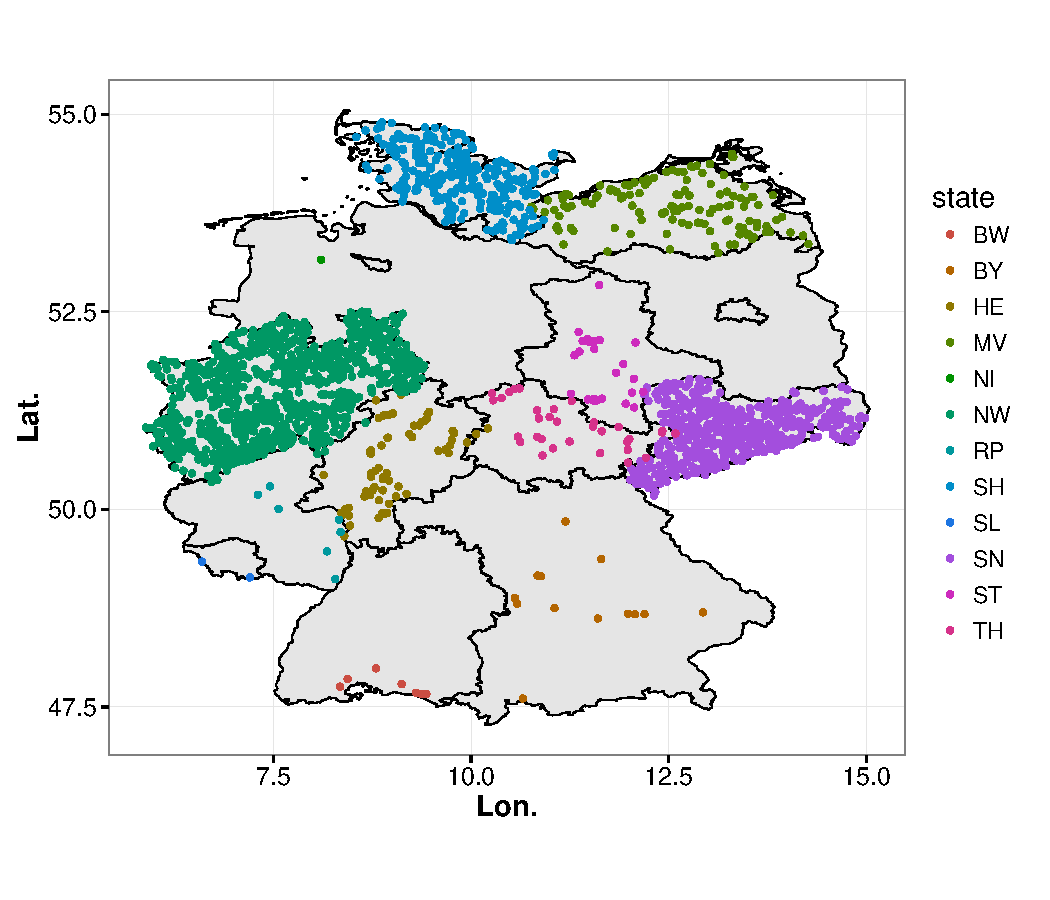
\includegraphics[width=0.6\textwidth]{figure1.pdf}
  \caption{Spatial distribution of the 3109 sampling sites. Colour codes different federal states.}
  \label{fig:fig1}
\end{figure}

In total 484 different compounds used as pesticides and their metabolites were measured at least once (Supplement, Table S2). 
Most of the compounds were herbicides (179), followed by insecticides (117) and fungicides (109).
We found substantial differences in the spectra of analyzed compounds between federal states (Figure \ref{fig:fig2} and Supplement Figure S2).
Hierarchical clustering revealed three groups:
i) with less then 100 compounds (SL, ST and TH), \\
% * <ralf.schaefer@aggiemail.usu.edu> 2016-08-27T14:06:20.935Z:
%
% gibt es irgendwo eine übersicht der bundesländer im ANhang? Sonst sind die abkürzungen kaum nachvollziebar. Sie könnten zudem in Fig 1 hinzugefügt werden
%
% ^.
ii) with medium sized spectra and \\
iii) with a big and distinct spectrum (RP and NI).

Only 5.5\% (160,800) of all measurements were detects above the limit of quantification (LOQ).
The spatio-temporal intersection revealed that 5\% of the samples were taken at or after days with rainfall events greater than 10mm / day (Supplement, Figure S3).

\begin{figure}[ht]
  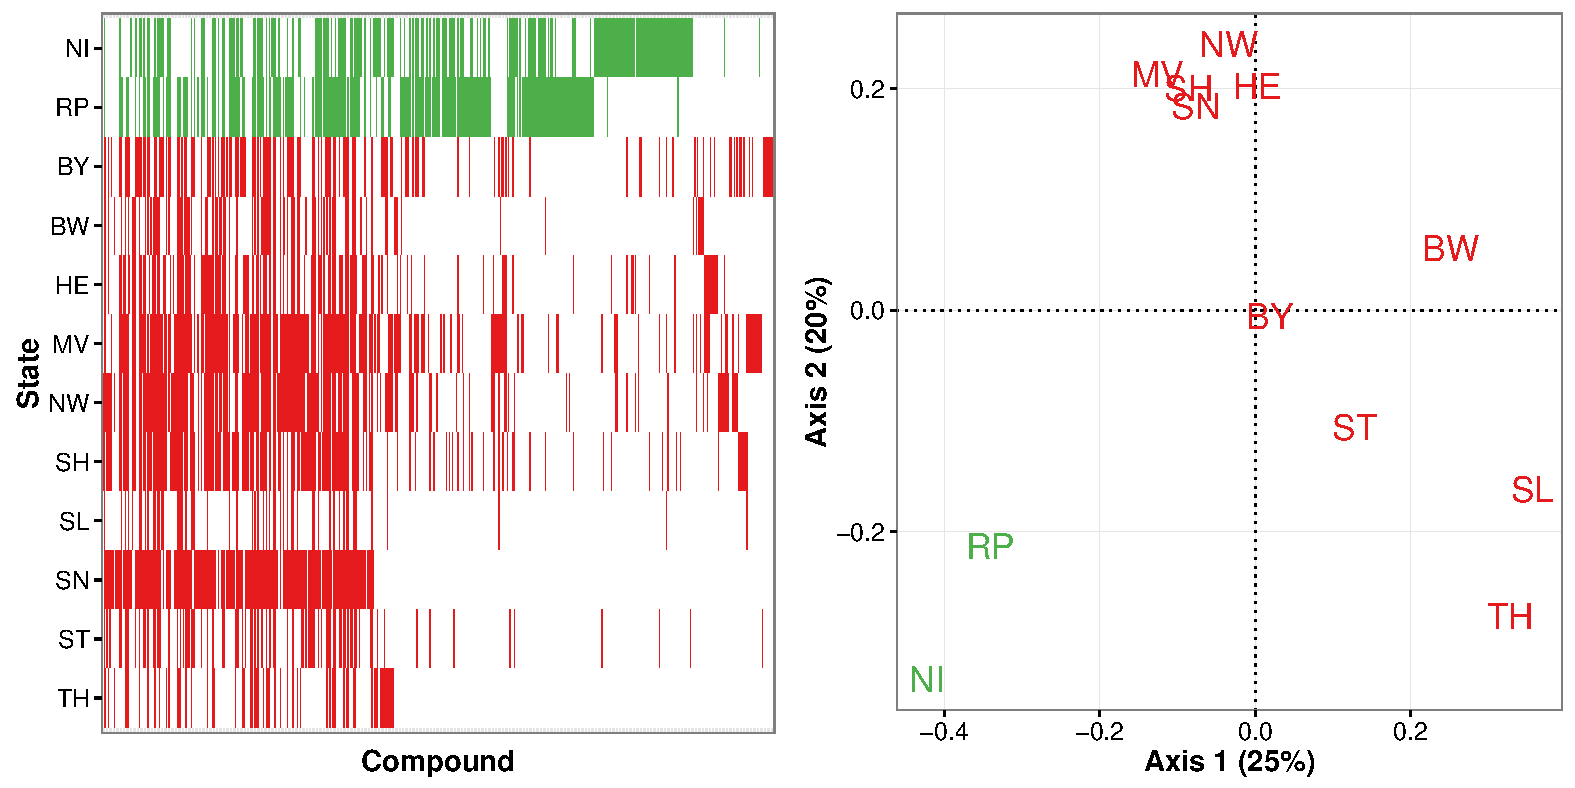
\includegraphics[width=\textwidth]{figure2.pdf}
  \caption{Compound spectra of the different federal states. Left: Barcode plot - Each vertical line is an analysed compound. Right: MDS ordination. 
  Colors according to three groups determined by hierarchical clustering (see Supplement Figure xxx).}
  \label{fig:fig2}
\end{figure}

We were able to derive for 2376 sites catchment sizes and the proportion of agriculture within catchments. 
% * <ralf.schaefer@aggiemail.usu.edu> 2016-08-27T14:09:28.040Z:
%
% präzisieren: d.h. für die ging der delineation algorithm? Oder für die anderen hatten auch die BL nichts und die wurden dann ausgeschlossen?
%
% ^.
The distribution of sampling sites across catchment area and agricultural area in the catchment revealed a sharp decline in the distribution of catchment-sizes below $10~km^2$, with most sampling sites with catchments between 10 and 25 $km^2$ (Figure \ref{fig:fig3}).
The proportion of agriculture in the catchments decreased with increasing catchment size.

\begin{figure}[ht]
  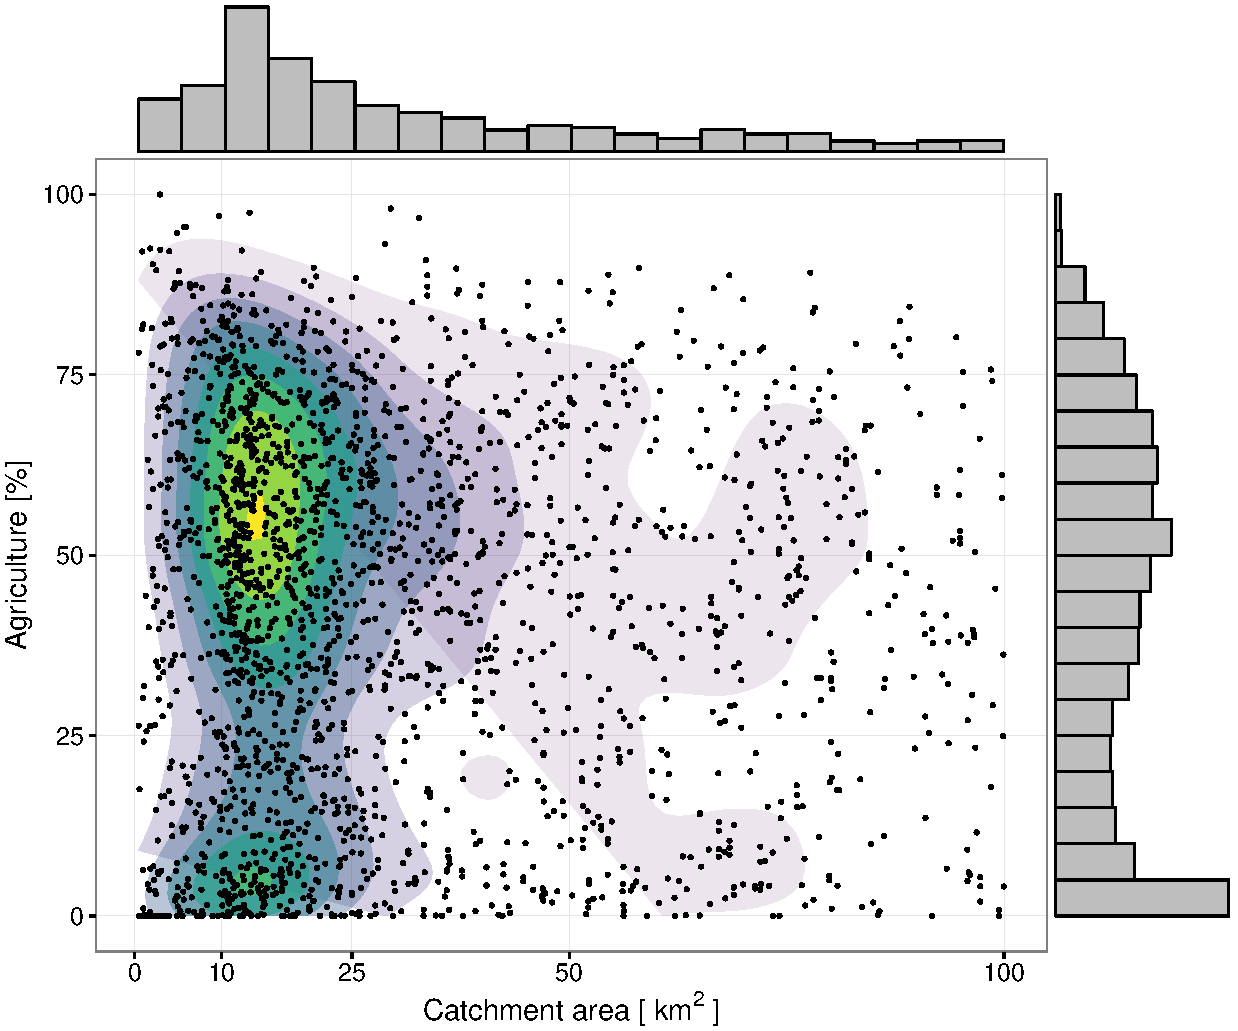
\includegraphics[width=.8\textwidth]{figure3.pdf}
  \caption{Distribution of catchment area and agriculture within the catchment area across the sampling sites.
  Only sampling sites with catchment area < 150 km\textsuperscript{2} are displayed. 
  Colour codes the 2-dimensional density of points.
  }
  \label{fig:fig3}
\end{figure}



\subsection{Are small agricultural waters more polluted compared to bigger streams?}

Modeling the number of RAC exceedances as function of agriculture within catchment and catchment size revealed that there is a strong and statistically significant increase up to 25\% agriculture.
Above this threshold the exceedances level off followed by a increase above 75\% (Figure \ref{fig:fig4}, left).

We could no detect any effect of catchment size on the number of RAC exceedances (Figure \ref{fig:fig4}, right) and no interaction between these two predictors.

\begin{figure}[ht]
  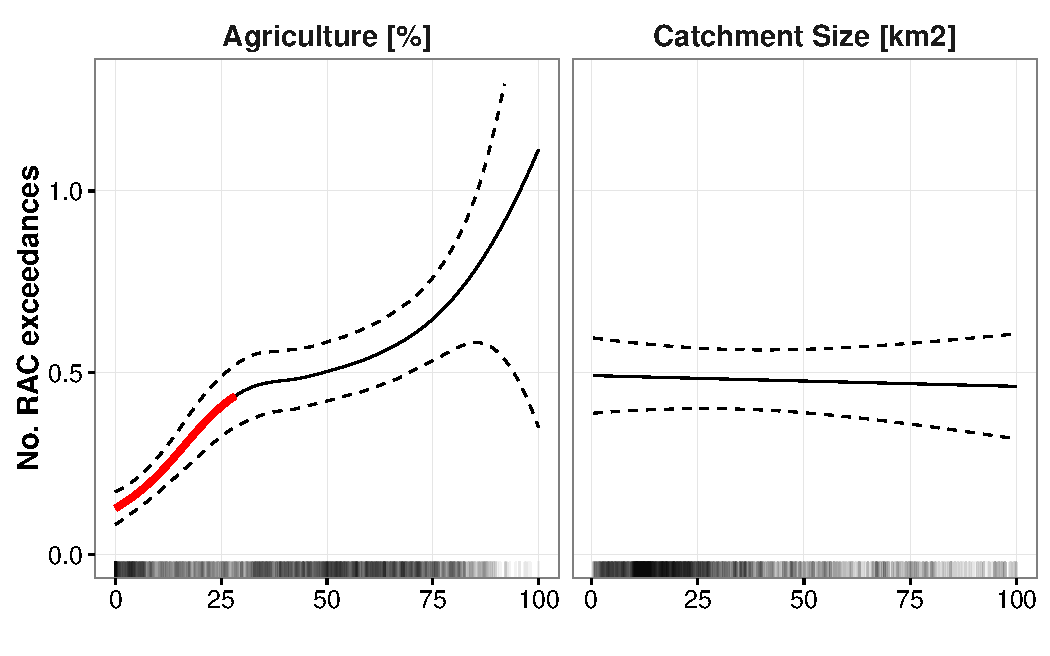
\includegraphics[width=0.95\textwidth]{figure4.pdf}
  \caption{Effect of agriculture within the catchment (left) and catchment size (right) on the number of RAC exceedances. Red line marks statistically significant changes. Dashed lines denote 95\% pointwise Confidence Intervals.
  }
  \label{fig:fig4}
\end{figure}

The number of EQS-exceedances and the 95th percentile of $TU_{max}$ showed similar patterns and thresholds (see Supplement, Figures S4-S8). 
% * <ralf.schaefer@aggiemail.usu.edu> 2016-08-27T14:16:26.707Z:
%
% Die fragen die hier beantwortet wird ist doch eher how is pesticide pollution connected with agricultural catchment cover and stream size? in der introduction wird auch wenig dazu gesagt, was jetzt das neue/innovative ist. Das wäre aber wichtig, wenn man es wie bei höheren journals wie ES&T unterbringen will
%
% ^.

\subsection{Pollution of small agricultural streams}
Based on the results and given the low amount of sample sites with catchment sizes below 10 km\textsuperscript{2} we explored the pollution of small agricultural streams, defined as streams with catchment size less than 30 km\textsuperscript{2} and more than 25\% agriculture within the catchment (n = 1030 sites with 10591 samples and 36550 measurements).
% * <ralf.schaefer@aggiemail.usu.edu> 2016-08-27T14:56:26.821Z:
%
% unklar, warum das hier genannt wird - ist ja nirgendwo vorher gesagt worden, dass genau die betrachtet werden sollten...
%
% ^ <ralf.schaefer@aggiemail.usu.edu> 2016-08-27T14:59:43.735Z:
%
% sieht auch eher so aus, als wenn - aber nicht signifikant) - im mittel die RAK überschreitungen stark zunehmen mit der Catchment size... Also doch eigentlich kein Hinweis, dass kleinere belastet sind? Würde es ggf. sinn machen bei der abbildung mit catchment size (Fig4.) bei 150 abzuschneiden, die Figure 3 geht auch nur bis 150)
%
% ^.
%EQS
% * <ralf.schaefer@aggiemail.usu.edu> 2016-08-27T15:02:38.601Z:
%
% der ganze abschnitt bezieht sich auf Pollution, aber eigentlich geht es nur darum, welche Substanzen relevant sind und nicht wie häufig überschreitungen auftreten. Überhaupt fragt man sich, warum genau diese Gruppe analysiert wird, da ja ggf. die größeren Gewässer nach der Darstellung hier anscheinend größer belastet sind?! (liegt ggf an der interaktion landwirtschaft und size?)
%
% ^.
Out of the 29 compounds with EQS, the most frequent EQS exceedances were recorded for the herbicides Nicosulfuron (2.1\%, n = 1769), Flufenacet (1.1\%, n = 6301) and Isoproturon (0.7\%, n = 8380). 
% * <ralf.schaefer@aggiemail.usu.edu> 2016-08-27T15:04:43.052Z:
%
% es wäre insgesamt auch ganz gut zu wissen, an wie viel % der stellen überhaupt irgendwas überschritten wurde
%
% ^.
Other compounds show exceedances only at less then 0.5\% of all samples (Figure \ref{fig:fig5}A).
% RAC
Neonicotinoid Insecticides and Chlorpyrifos showed highest risk quotients.
For Thiacloprid, Imidacloprid and Chlorpyrifos RAC was less than LOQ, therefore, all detections have a RQ \textgreater 1 (Figure \ref{fig:fig5}B). 
In 15\% of all samples (n = 6377) risk quotients higher then 1 were observed.
Highest RQ were observed for Chlorpyrifos (244), Dimoxystrobin(117) and Isoproturon (80). 
% TU
In 33\% of the samples no pesticides were detected. 
The mean $log_{10}(TU_{max})$ for detects was -4.6.
2.6\% of the samples showed $log_{10}(TU_{max})$ values greater then -2 (Figure \ref{fig:fig5}C).
% * <ralf.schaefer@aggiemail.usu.edu> 2016-08-27T15:07:14.707Z:
%
% Figure 5 kann ich nicht sehen
%
% ^.
We found a high correlation of $log_{10}(TU_{max})$ and $log_{10}(TU_{sum})$ (r = 0.985, with a maximum higher value of $log_{10}(TU_{sum})$ of 0.75 units (Supplement, Figure S9).
% * <ralf.schaefer@aggiemail.usu.edu> 2016-08-27T15:07:36.663Z:
%
% wenn man das in den Risk assessment kontext stellen will, was ja schwierig ist, dann müsste in der einleitung das besser vorbereitet werden.
%
% ^.
% see do_polluion.R for numbers
%Mixtures
In most samples (55.5\%) more then one compound was detected, with a maximum of 54 different compounds (Figure \ref{fig:fig5}D). 

%% Add more numbers / percentages here => compare with knauer/stehle/Vijver

\begin{figure}[h]
  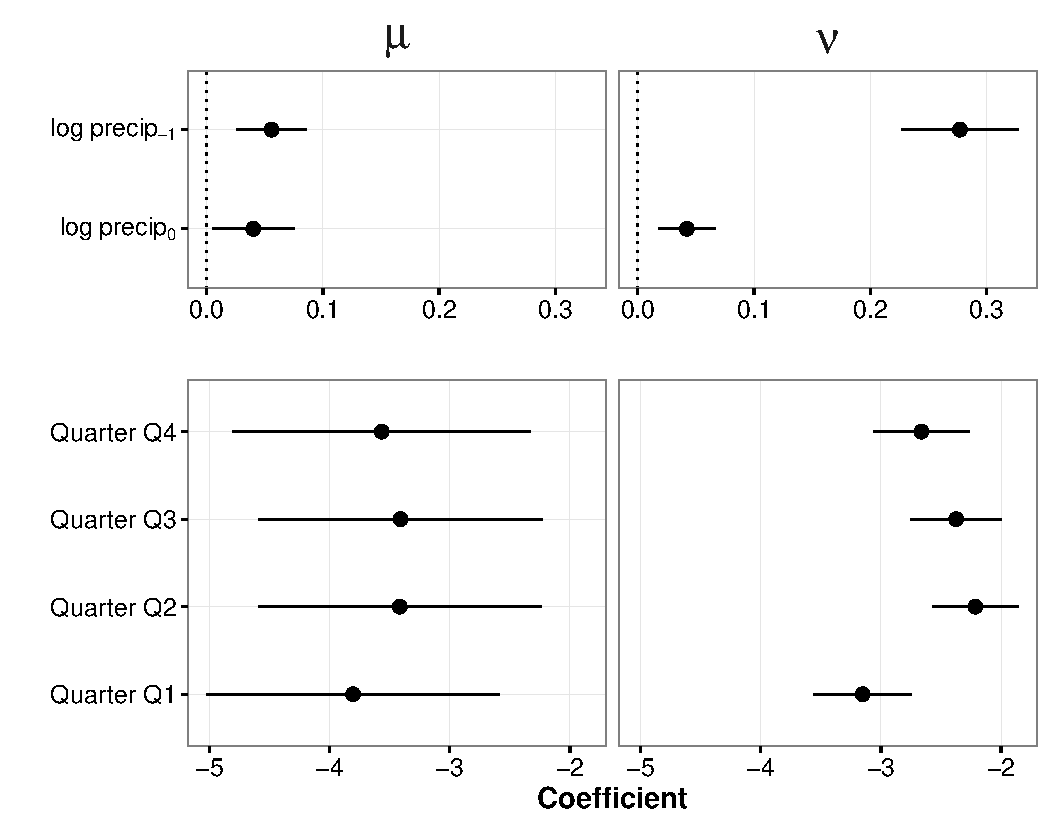
\includegraphics[width=0.9\textwidth]{figure5.pdf}
  \caption{Overview on pesticide pollution of small agricultural streams (catchment size \textless 30 km\textsuperscript{2} and \textgreater 25\% agriculture). 
      \textbf{A}: 10 compounds with most frequent EQS exceedances. See B for color legend.
      \textbf{B}: Distribution of $TU_{max}$ values. Values with $TU_{max} = 0$ are not displayed (3501 out of 10591 samples). Non-detects are not shown due to the logarithmic axis.
      \textbf{C}: 15 compounds with highest risk quotients. Non-detects are not shown due to the logarithmic axis.
      \textbf{D}: Distribution of the number of detected compounds in a sample.
  }
  \label{fig:fig5}
\end{figure}

% * <ralf.schaefer@aggiemail.usu.edu> 2016-08-27T15:13:15.860Z:
%
% was ist denn mit den Regendaten, die tauchen gar nicht mehr auf
%
% ^.

\section{Discussion}
\subsection{Overview on the compiled dataset}
The compiled dataset of governmental monitoring data represents currently the most comprehensive one available for Germany.
Similar nationwide datasets have been compiled for the Netherlands \citep{vijver_spatial_2008}, Switzerland \citep{munz_pestizidmessungen_2011} and the United States (Water Quality Portal (WQP) \url{www.waterqualitydata.us}).
The data compiled here for Germany is of similar quantity and quality.
% * <ralf.schaefer@aggiemail.usu.edu> 2016-08-27T15:09:01.348Z:
%
% and analysed? 
%
% ^.

% current problems in monitoring and possible solutions
Nevertheless, a nationwide assessment of pesticide pollution is hampered by the inhomogeneity of monitoring data between federal states:
There are not only big differences in the spatial distribution and quantity of sampling sites (Figure \ref{fig:fig1}), but also the spectrum of analyzed compounds (Figure \ref{fig:fig2}) and differences in the quality of chemical analyses. 
% * <ralf.schaefer@aggiemail.usu.edu> 2016-08-27T15:11:28.611Z:
%
% klar - aber je nach fragestellung könnte man sich nur auf die Substanzen beziehen, die überall gemessen werden. Was mit repräsentativ überhaupt gemeint ist, ist nicht überzeugend im artikel dargelegt und warum das wichtig ist... ich denke, hier können wir mal diskutieren, was denn die hauptfrage ist: Kann man mit monitoringdaten repräsentatives assessment machen? Das scheitert ja alleine schon am grab sampling und ist somit von vornherein beantwortet. Oder welche fragen man nur mit großen datensätzen beantworten kann.
%
% ^.
An increase of the analyzed compound spectra to all registered compounds and a lowering of LOQ are desirable for a reliable assessment.
% * <ralf.schaefer@aggiemail.usu.edu> 2016-08-27T15:13:49.591Z:
%
% umgekehrt wird aber gesagt, dass eigentlich nur ein paar substanzen relevant sind - so richtig begründet erscheint diese forderung nicht...
%
% ^.
Our dataset comprised several thousand stream sampling sites, but nearly no data could be compiled for standing waters. 
% * <ralf.schaefer@aggiemail.usu.edu> 2016-08-27T15:14:41.955Z:
%
% das ist für das projekt relevant, aber man fragt sich, was das hier soll. Ich würde die von vornherein rausschmeißen und sagen, dass das monitoring vor allem auf fließgewässer bezogen ist
%
% ^.
Although, standing waters are abundant in the agricultural landscape and may have a high contribution to biodiversity \citep{davies_comparison_2008}, nearly nothing is known on their chemical status.
Small streams comprise most of the total stream length \citep{nadeau_hydrological_2007}.
However, sampling sites with catchment sizes below $10km^2$ are underrepresented by the current monitoring scheme (Figure \ref{fig:fig3}).
This likely arises because catchments under $10km^2$ are not specified by the WFD.
% * <ralf.schaefer@aggiemail.usu.edu> 2016-08-27T15:15:49.749Z:
%
% hä?? Die sind nicht berichtspflichtig, aber die behörden gehen davon aus, dass die anforderungen des guten ökologischen zustands auch für diese gewässer gelten
%
% hä?? Die sind nicht berichtspflichtig, aber die behörden gehen davon aus, dass die anforderungen des guten ökologischen zustands auch für diese gewässer gelten
%
% ^.
Nevertheless, small streams should not be neglected for ecological and chemical quality assessment.
Future monitoring programs should aim at resolving these issues in order to enable a nationwide and representative assessment of freshwaters. 
% * <ralf.schaefer@aggiemail.usu.edu> 2016-08-27T15:16:47.488Z:
%
% ich denke, dass kann hier eher ein untergeordneter aspekt sein
%
% ^.

% underestimation
Given the fixed term monitoring design \citep{stehle_probabilistic_2013} and the low amount of samples taken at precipitation events that could lead to run-off, the data represents a underestimation of the real pollution and peak concentrations.
% * <ralf.schaefer@aggiemail.usu.edu> 2016-08-27T15:20:23.131Z:
%
% das wird doch gar nicht gezeigt bzw. dargelegt, dass das underestimated ist... bzw. ist das kein ergebnis dieser studie nach aktueller lage
%
% ^ <ralf.schaefer@aggiemail.usu.edu> 2016-08-27T15:21:08.769Z:
%
% also mit lage meine ich im text
%
% ^.
Automatic event-drive samplers and passive samplers may help overcome these shortcomings and provide a better representation \citep{fernandez_calibration_2014,moschet_evaluation_2015}.
Nevertheless, such nationwide compilations, may not only be used for governmental surveillance, but also to answer other questions, like validation of exposure modeling \cite{knabel_fungicide_2014}, retrospective evaluation of regulatory risk assessment \citep{knauer_pesticides_2016,stehle_pesticide_2015}or occurrences of pesticide mixtures \cite{schreiner_pesticide_2016}.


\subsection{Influence of catchment area and agriculture}
% agriculture
We found a strong influence of agriculture on the pollution of streams.
If there is more the 25\% agriculture within a catchment pesticides can generally be detected in streams with an increase in fully agricultural catchments (above 75 \% agriculture).
% * <ralf.schaefer@aggiemail.usu.edu> 2016-08-27T15:21:56.186Z:
%
% unklar, wo das genau gezeigt wird - die anzahl der detektionen gegen %catchment wird nicht gezeigt...
%
% ^.
To our knowledge this is the first study \todo{True? Could not find anything...} investigating such thresholds of pesticide occurrences.
% * <ralf.schaefer@aggiemail.usu.edu> 2016-08-27T15:22:35.375Z:
%
% denke auch - aber man müsste hier 2-3 Studien nennen, die ich im Abschlussbericht zitiert habe, die ähnliche thresholds gefunden haben und könnte sagen, dass unsere studie insofern nahelegt, dass der faktor pestizide auch relevant ist
%
% denke auch - aber man müsste hier 2-3 Studien nennen, die ich im Abschlussbericht zitiert habe, die ähnliche thresholds gefunden haben und könnte sagen, dass unsere studie insofern nahelegt, dass der faktor pestizide auch relevant ist
%
% ^.
Our results suggest that only catchments with \textless 25\% agriculture may be regarded as unpolluted and could be used as reference sites.
% * <ralf.schaefer@aggiemail.usu.edu> 2016-08-27T15:24:08.697Z:
%
% das ist mir in fig. 4 nicht ganz klar. Wenn das immer point estimates sind, die signifikant sind, dann wären ja schon 5% höher als 1%, weil ja die ganze linie bis 25% rot ist. Oder wie ist das zu lesen? Insofern kann man auch schlecht sagen auf basis des fast linearen anstiegst, dass 20% genauso ist wie 2%
%
% ^.
Slightly higher thresholds (20-40\%) have been found for biological responses of lotic assemblages to land-use \citep{waite_agricultural_2014, feld_response_2013}, though there might be differences between taxonomic groups and landscape \citep{feld_response_2013}.
% * <ralf.schaefer@aggiemail.usu.edu> 2016-08-27T15:26:50.631Z:
%
% das würde genauerer Diskussion bedürfen, denn das sagt dann ja, dass für Diatomeen oder invertebraten und für die unterschiedlichen bundesländer unterschiedliche % zahlen relevant sein könnten. Könnte man ja eh überprüfen
%
% ^.
% * <ralf.schaefer@aggiemail.usu.edu> 2016-08-27T15:26:07.465Z:
%
% land use ist doch gar nciht relevant - nur spezifisch agriculture
%
% ^.
% * <ralf.schaefer@aggiemail.usu.edu> 2016-08-27T15:25:37.776Z:
%
% 20% ist nicht higher...
%
% 20% ist nicht higher...
%
% ^.

% size
We did not find support for our hypothesis that small streams are more polluted than big streams, though previous studies have show such a relationship \citep{schulz_field_2004,stehle_pesticide_2015,knauer_pesticides_2016}.
% * <ralf.schaefer@aggiemail.usu.edu> 2016-08-27T15:28:35.191Z:
%
% kannst du mir knauer mal schicken?
%
% ^.
% * <ralf.schaefer@aggiemail.usu.edu> 2016-08-27T15:28:05.039Z:
%
% ist nicht als hypothese formuliert vorher
%
% ^.
This could be explained by the relatively short gradient of catchment sizes in our dataset, with most of the streams being \textless $100~km^2$ (Figure \ref{fig:fig3}, top).
For example the gradient of \citet{schulz_field_2004} covered 6 orders of magnitude.
% * <ralf.schaefer@aggiemail.usu.edu> 2016-08-27T15:30:08.003Z:
%
% indeed - so richtig kann man das nicht testen und die definition von "big" dürfte einige verwundern
%
% ^.
Another reason might be the the unequal distribution of catchment sizes, with less sites \textless $10~km^2$ and \textgreater $100~km^2$ (Figure \ref{fig:fig3}, top).


\subsection{Pollution of streams}
% RAC
\citet{stehle_pesticide_2015} found the highest percentage of RAC exceedances for organophosphate insecticides. 
By contrast, our results revealed that neonicotinoid insecticides show high exceedances, followed by the organophosphate chlorpyrifos. 
This difference can be attributed to the low sample size for neonicotinoid insecticides in their study (n = 33) compared to the dataset presented here (n = 3516-4745) and shows that this particular class of insecticides may currently pose a high risk to freshwater ecosystems.
% * <ralf.schaefer@aggiemail.usu.edu> 2016-08-27T15:31:58.251Z:
%
% unklar warum spanne
%
% ^.
Our results show lower proportions of exceedances compared to \citet{stehle_pesticide_2015}, which can be attributed to different aims of the data sources: scientific research aims at finding pollutants, whereas monitoring aims mainly at surveillance of water quality, also during periods with lower pesticide usage. 
% * <ralf.schaefer@aggiemail.usu.edu> 2016-08-27T15:34:37.233Z:
%
% wo???
%
% ^.
This is also reflected in the different sample sizes (1,566 vs. 1,117,988 measurements of compounds with RAC) and the high number of non-detects in the monitoring data.
% * <ralf.schaefer@aggiemail.usu.edu> 2016-08-27T15:35:13.107Z:
%
% unklar
%
% ^.
Contrary, \citet{knauer_pesticides_2016} found exceedances from monitoring data mainly for herbicides and fungicides and only one insecticide Chlorpyrifos.
This might reflect differences in pesticide use between countries and defined RACs.
% * <ralf.schaefer@aggiemail.usu.edu> 2016-08-27T15:36:00.776Z:
%
% was überhaupt mal gebracht werden sollte ist der bezug von RAC zu biodiversität - dafür kann ja Stehle & Schulz dienen?
%
% ^.
For three insecticides all detected values where above the RAC.
This highlights that national monitoring programs need to improve chemical analytics and lower the LOQ for these highly toxic compounds.

% TU
8.2\% of samples showed $TU_{max}$ values greater than -3 (Figure \ref{fig:fig5}C), a threshold above which ecological effects have been shown \citep{schafer_thresholds_2012}.
This suggests that pesticides may act as a common stressor to freshwaters and should not be neglected \citep{schafer_contribution_2016}.
% * <ralf.schaefer@aggiemail.usu.edu> 2016-08-27T15:37:12.651Z:
%
% by what or whom? The monitoring shows that they are taken serious?!
%
% ^.
The high correlation of TU and the relatively low increase of $TU_{sum}$ reveals that in compound mixtures occurring in the field there is a skewed distribution of toxicities with mainly one compound dominating the toxicity.
% Mixtures
Nevertheless, most pesticides did not occur individually but in mixtures \cite{schreiner_pesticide_2016} and future risk assessment should take mixtures into account.
% * <ralf.schaefer@aggiemail.usu.edu> 2016-08-27T15:37:54.188Z:
%
% problem der bestimmung ist doch hier auch relevant. SIehe die Moschet studien. ob dazu gezielter was zu sagen, müsste man mal stellen nach regen und vielen substanzen mit anderen vergleichen, was die sumTox angeht
%
% ^.

% EQS
For only a limited number of compounds EQS have been defined. 
We found generally low exceedances of EQS with only three herbicides showing higher exceedances.
However, compared to the results from RAC comparisons it is clear that the currently defined EQS cannot capture the full risk exposed by pesticides.
In order to provide a reliable measure of a good chemical status EQS for additional compounds must be defined.
% * <ralf.schaefer@aggiemail.usu.edu> 2016-08-27T15:39:15.216Z:
%
% was trägt EQS eigentlich insgesamt zur Story bei? Ist mir nicht ganz klar. Gibt kaum Ergebnisse hierzu und für 30 von 400 substanzen was zu machen, ist auch nicht so überzeugend
%
% ^.

% Approval / Risk Assessment
Monitoring data, despite the outlined limitations, provides an opportunity to study environmental occurrences of pesticides after approval.
The high exceedances of RAC indicate that the approval process for pesticides must be checked and refined.




%%%%%%%%%%%%%%%%%%%%%%%%%%%%%%%%%%%%%%%%%%%%%%%%%%%%%%%%%%%%%%%%%%%%%
\begin{acknowledgement}
The authors thank the federal state authorities for providing chemical monitoring data and the German Federal Environmental Protection Agency (UBA) for funding a related project. 
% * <ralf.schaefer@aggiemail.usu.edu> 2016-08-27T15:40:29.902Z:
%
% typischerwiese wird dann die projektnummer angegebn
%
% ^.
\end{acknowledgement}


%%% Word count
% abstract    :
% 3 big(600)  : 1800
% 2 small(300): 600
% text body   : 3000 
% ackno       : 24
% ======================================
% total       : 

%%%%%%%%%%%%%%%%%%%%%%%%%%%%%%%%%%%%%%%%%%%%%%%%%%%%%%%%%%%%%%%%%%%%%
\begin{suppinfo}
The following files are available free of charge.
\begin{itemize}
  \item Supplemental\_Materials.pdf : Supplemental Materials (Figures, Tables, Models).
\end{itemize}
\end{suppinfo}
% * <ralf.schaefer@aggiemail.usu.edu> 2016-08-27T15:41:32.807Z:
%
% ok - jetzt habe ich erst fig 5 gefunden... macht ggf. den ein oder anderen kommentar überflüsig
%
% ^.


%%%%%%%%%%%%%%%%%%%%%%%%%%%%%%%%%%%%%%%%%%%%%%%%%%%%%%%%%%%%%%%%%%%%%
\bibliography{references}

\end{document}
